\documentclass[12pt]{article}

\usepackage{fontspec}
\usepackage{graphicx}
\usepackage{wrapfig}
\graphicspath{ {images/} }

\title{Sluttraport praksis i arbeidslivet - DAT156}
\date{Haust 2017}
\author{Sigurd Gravning \\146188 \\ \\Wide Assessment \\Stine Andreassen}

\begin{document}

\maketitle
\pagenumbering{gobble}
\newpage
\pagenumbering{arabic}
\tableofcontents
\newpage

\section{Intro}

Når eg var i prosessen med å finna praksisplass til dette semesteret vart eg så
heldig å komma på intervju med både Sparebanken Vest, og Wide Assessment.
Dette gav meg ein unik moglegheit til å velga mellom to vidt forskjellige firma,
og vidt forskjellige erfaringar. Intervjuet med Wide Assessment var kort, konsist,
og rett på sak. I motsetning til intervjuet med SPV, som var lengre og meir forvirrande,
sidan dei ikkje hadde hatt elevar til praksis før. Etter litt tid fekk eg
tilbakemeldig frå SPV, som sa dei ikkje var klare for å ta inn nokon i praksis
dette semesteret. So då begynte samtalen med Stine frå Wide Assessment med ein gong.
Eg starta  i praksis der med ein gong semesteret starta, og eg må sei eg er glad
for at det blei Wide Assessment i staden for SPV. Eg håpte personleg å lære ein
del om arbeidslivet og få oppleva korleis det vil vera når ein kjem ut i jobb.
Som ein student som har sete på skulebenken i 17 år, var det veldig forfriskande
å sjå kva ein skal jobba med. Som eg trudde var det også mykje nytt ein ikkje
lære på Høgskulen som er viktig ute i arbeidslivet. Wide Assessment har vert
ein veldig ideell praksis plass med nok å gjera, og hyggelege folk som alltid
er villige til å hjelpa. 

\section{Wide Assessment}

Wide Assessment er eit lite oppstartsfirma, beståande av Stine Andreassen,
Arve Andreassen, Eivind Hjertnes, Viljar Rolfsen, og Andreas Hammerbeck.
Hovudproduktet deira er wa.works, ei nettside som gjer da lettare for jobbsøkarar
og bedrifter innan tech å finna kvarandre. Som ein jobbsøkar leggar ein inn CV'en
sin, men får også vurdert eigenskapane sine i forskjellige språk og teknologiar
som er aktuelt i tech bransjen. Då får bedrifter ein mykje betre innsikt over
kva ein kandidat faktisk kan og har jobba med enn det som står i ein CV.
Idéen byrja når Stine leita etter ein ny jobb og jobba gratis for Arve i Gyril.
Gyril er eit rekruteringsfirma Arve har vert med å starte opp. Her brukte han
eit excel ark til skill assessment for jobbsøkarar. Dette blei basisen for Wide
Assessment ved å forenkla prosessen og få det som ein nettløysing. Stine og Arve
fekk fort støtte frå Innovasjon Norge, og fekk bekrefta at dette var ønska av å
gjera markedsundersøkingar. Sjølve prosjektet starta i Mars 2015 og dei blei ein
bedrift April 2016. I starten tok dei mykje bruk av studentar og nyutdanna frivillige
for å bygga grunnmuren. Her blei det bestemt mykje om korleis "produktet" skulle
sjå ut. I November 2016 blei Eivind ansatt som sjefs utviklar, der dei gjekk frå
Angular til React. Når det gjaldt innhenting av kapital so gjekk dette over all
forventning. Noko som førte til at dei fekk eit oppstartslån frå Innovasjon Norge
i Mars, som også førte til Viljar sin ansettelse. Andreas var først vurdert til
denne stillingen, men valgte å gå vidare på ein Master, so han har heller blitt
ansatt i ein deltidsstilling. På grunn av at Arve er for augenblikket ansatt i
Gyril, har WA 3 og ein halv ansatte, men 4 og ein halv er på teamet. Sidan det går so
bra, vil Arve mest sannsynleg bli ansatt i Februar - Mars.

\section{Arbeidsforhold}

Wide Assessment er del av Bergen Works, som er ein samla arbeidsplass for ein
handfull innovative firma i Bergen. Her er det opent kontorlandskap og felles
lunsj, so ein blir fort kjend med mange av dei forskjellige folka som jobbe der.
Innad i Wide Assessment var da veldig lågt under taket for å stilla spørsmål heilt
frå starten av. Både Viljar som utviklar og Eivind som sjefsutviklar var hjelpsame
når ein hadde noko som helst problem med da ein jobba med. Det føltes desverre ikkje
lika lett i starten å spørra om hjelp. Bergen Works var i prosessen å flytta lokale
til det store opne landskapet dei er i no. So me hadde ikkje plass til at me i
praksis kunne sitta i same rom som dei fast ansatte.

\begin{figure}[h]
  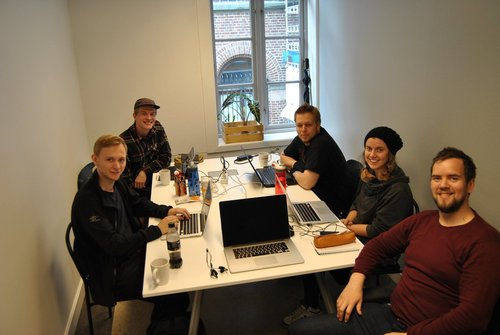
\includegraphics[width=0.75\textwidth]{Studenter}
  \centering
\end{figure}

Stine, som er leiar i Wide Assessment, har vert veldig aktiv med oss.

\end{document}
